\documentclass{article}
\usepackage{graphicx}
\usepackage{caption}
\usepackage{subcaption}
\usepackage[paper=a4paper,margin=1in]{geometry}
\usepackage[fontsize=12pt]{fontsize}
\usepackage{amsmath, amsthm, amssymb}
\usepackage[hidelinks]{hyperref}
\usepackage[nameinlink, noabbrev]{cleveref}

\newtheorem{theorem}{Theorem}[section]
\DeclareMathOperator{\sgn}{sgn}

\title{Math 475 -- Project 1 \\ Bobcat Population}
\author{Jackson Brienen}
\date{October 8 2025}

\begin{document}

\maketitle

\section{Introduction}
In this paper we discuss how we can model bobcat populations under a variety of environmental conditions and external manipulations (hunting and introduction). While there are a variety of modeling techniques that can be used for populations we focus on using a basic exponential model. With this come a variety of assumptions:

\begin{enumerate}
    \item There is no carrying capacity/ maximum population.
    \item The growth rate of the population is always constant, i.e. the growth rate in the first year will be the same as the hundredth year, and thousandth year, and so on.
    \item We assume, in most cases, that fractional populations are valid. While one half of a bobcat does not usually make sense, for the sake simplicity we will allow it to be the case unless we explicitly say we use integer based populations.
    \item All births and deaths happen at the end of a year/ start of a new year.
    \item All time increments, denoted $t$ throughout the paper, are integers greater than or equal to zero.
    \item Any $P(0)$, i.e. initial population will be greater than zero, throughout the paper we usually use $P(0)=100$.
\end{enumerate}

This paper will be divided into three main topics. First, the analysis of the basic model under three different growth rates in both the long and short term. Second, we will how the model changes when hunting is introduced and devising a strategy to meet a stable population with hunting. Third and last, we will analyze how the model changes when external introduction is used along with devising a strategy to meet a stable population with introduction.

\section{Methods}
When analyzing the different models in this paper we use a variety of mathematical techniques and definitions to predict and describe their behavior. While understanding the exact underlying mathematics can be helpful, understanding general terminology and theory is more important for reading this paper.

\subsection{Properties of Exponential Functions}
This paper exclusively discusses exponential functions. An exponential function $f(x)$ can fall into three categories:
\begin{itemize}
    \item Exponential Growth: $f(x)$ increases towards $\infty$.
    \item Exponential Decay: $f(x)$ decreases towards 0.
    \item Constant: $f(x)$ does not change.
\end{itemize}
When analyzing exponential functions we may want to know which category they fall into. While the derivative of $f(x)$ could be used, sometimes this derivative can be unpleasant. Since this paper focuses primarily on discrete recurrence which are exponential in their closed form, it is very easy to calculate the rate of change at a single point. We can then you the sign of this rate of change to determine its behavior (growth, decay, constant). To do this we must know that the sign of the rate of change of the function does not change. For this we can rely on the following theorem.

\begin{theorem}\label{thm:1}\normalfont
    Let $f(x)=a \cdot b^{cx+d} + e$ where $a, b, c, d, e \in \mathbb{R}$, the form for any defined exponential function. If $f(x)$ is defined $\forall x \ge 0$ the derivative $f'(x)$ will have the same sign for any $x \ge 0$.
\end{theorem}
\begin{proof}
    Let $f(x)=a \cdot b^{cx+d} + e$ where $a, b, c, d, e \in \mathbb{R}$. Assume $f(x)$ is defined $\forall x \ge 0$. We will show that $f'(x)$ is constant for all $x \ge 0$.\\
    We begin by taking the derivative of $f(x)$.
    $$
        f'(x) = ac \cdot b^{cx+d} \ln(b)
    $$
    The exponential term $b^{cx+d}$ will always have a positive sign, thus it can be removed when we calculate the sign of the derivative. With it removed we have a formula for the sign of $f'(x)$. 
    $$
        \sgn(f'(x))=\sgn(ab\ln(b))
    $$
    This leaves us with a few cases:
    \begin{itemize}
        \item[\textbf{Case}] $b = 0$. In this case $\ln(b)$ will be undefined, but our function becomes $f(x)=a \cdot 0^{cx+d} + e$, which in the cases where $x \ge 0$ we know $f(x)$ is defined, so this is equivalent $f(x) = a + e$ when $x \ge 0$. Since $f(x)$ is a constant, it's derivative is 0, and thus does not change signs.
        \item[\textbf{Case}] $0 < b < 1$. In this case $\ln(b)$ will be negative, since $b$ does not change, it will always be negative. So $\sgn(f'(x))=\sgn(ab\ln(b))$, will be constant.
        \item[\textbf{Case}] $1 < b$. In this case $\ln(b)$ will be positive, since $b$ does not change, it will always be positive. So $\sgn(f'(x))=\sgn(ab\ln(b))$, will be constant.
        \item[\textbf{Case}] $b < 0$. In this case $f(x)$ would not be defined for all $x \ge 0$. As for example, at $x = \frac{1}{2}$, $b^x = \sqrt{b} \notin \mathbb{R}$.
    \end{itemize}

    Therefore, we have shown that when $f(x)$ is defined for $x \ge 0$, $f'(x)$ will have a constant sign.
\end{proof}

\subsection{Finite Geometric Series Formula}
Sometimes, and in this paper, when we solve recurrence relations we are left with a finite geometric series. The finite geometric series formula in \cref{eq:geometric-series} allows for us to solve for a closed-form expression.
\begin{equation}\label{eq:geometric-series}
    \sum_{n=0}^{k}ar^n = \frac{a(r^n-1)}{r-1}, \text{ when } r \ne 1
\end{equation}

\subsection{Fixed Points} \label{sect:fixed-points}
Suppose we have a recursive function $x(n)=f(x(n-1))$. If $f(\bar{x}) = \bar{x}$, we say $\bar{x}$ is a fixed-point, and our system is in a stable state. We will discuss explicitly finding stable points later in this paper, as the stable point will be model dependent.

Fixed-points can be either stable (attractor) or unstable (repeller). A stable fixed-point means that if $x(n)$ starts either above or below the fixed-point, it will approach it. An unstable fixed-point means that if $x(n)$ starts above or below the fixed-point as $n$ increases $x(n)$ will get further from the fixed-point.

Classifying a fixed-point is fairly simple, if we let $\varepsilon(n)$ be the distance from a given fixed-point, $\varepsilon(n) = x(n) - \bar{x}$. We can then attempt to solve for the distance of the next $n$.
\begin{align*}
    \varepsilon(n) &= x(n) - \bar{x} \\
    \varepsilon(n+1) &= x(n+1) - \bar{x} \\
                  &= f(x(n)) - \bar{x} & \text{remember that } x(n)=f(x(n-1)). \\
                  &= f(\varepsilon(n) + \bar{x}) - \bar{x} & \text{by rearranging the initial equation}. \\
                  &\approx f(\bar{x}) + f'(\bar{x})\varepsilon(n) - \bar{x} & \text{through first-order Taylor expansion}\\
                  & &\text{assuming } \varepsilon(n) \text{ is close to 0}. \\
                  &= f'(\bar{x})\varepsilon(n) & \text{since } f(\bar{x})=\bar{x}.
\end{align*}
With this it follows that for a stable fixed-point, $\varepsilon(n+1)=f'(\bar{x})\varepsilon(n)$ should be shrinking as $n$ increases. This implies that for a stable fixed-point $|f'(\bar{x})| < 1$. And $|f'(\bar{x})| > 1$ for an unstable fixed-point. So, using the derivative of $f$ at our fixed-point, we can classify the fixed-point.


\section{Basic Growth}
This section discusses the basic growth model which we use throughout this paper. We start with a very basic recursive function $P(t)$ which takes our previous population $P(t-1)$ and adds the annual change to the population $rP(t-1)$, where $r$ is some growth rate. This simplifies to \cref{eq:basic-recursive-exponential}.

\begin{equation} \label{eq:basic-recursive-exponential}
    P(t) = (r+1)P(t-1)
\end{equation}

Previously we mentioned we were using an exponential model, yet this recursive formula does not look exponential. While it might not be immediately obvious, we can solve the recurrence for its closed form expression.

\begin{align}\label{eq:basic-closed}
    P(t) &= (r+1)P(t-1) & P(t-1) &= (r+1)P(t-2) \nonumber \\
    P(t) &= (r+1)\left((r+1)P(t-2)\right) & P(t-2) &= (r+1)P(t-3) \nonumber \\
    P(t) &= (r+1)\left((r+1)\left((r+1)P(t-3)\right)\right) & P(t-3) &= (r+1)P(t-4) \nonumber \\
    &\phantom{x}\vdots \nonumber \\
    P(t) &= (r+1)^tP(0)
\end{align}

In this closed form we can see clearly that this is in fact an exponential model. We can predict how the model will behave by using \cref{thm:1}. All we need to calculate is the change in population from one year to the next, we will use time at $0$ and $1$.
\begin{align*}
    P(1) &= (r+1)P(0) & \text{to get the change we simply find } P'(1)=P(1)-P(0)\\
    P'(1) &= (r+1)P(0)-P(0) \\
    P'(1) &= rP(0) + P(0) - P(0) \\
    P'(1) &= rP(0)
\end{align*}
Know that we know our change, we need to find the sign of this. As stated in the assumptions we know $P(0)>0$, so this is a positive constant, thus $\sgn(P'(1)) = \sgn(r)$, and by \cref{thm:1} we know our sign never changes, so $\sgn(P'(n))=\sgn(r)$. So we know that if $r > 0$ we will experience exponential growth, and if $r < 0$ we will experience exponential decay.


There are three growth rates based on environmental conditions, $1.676\%$ in the best case, $0.549\%$ in moderate cases, and $-4.5\%$ in the worst case, we will look at these when the starting population is $100$.

\begin{figure}[h]
    \centering
    \begin{subfigure}{.5\textwidth}
        \centering
        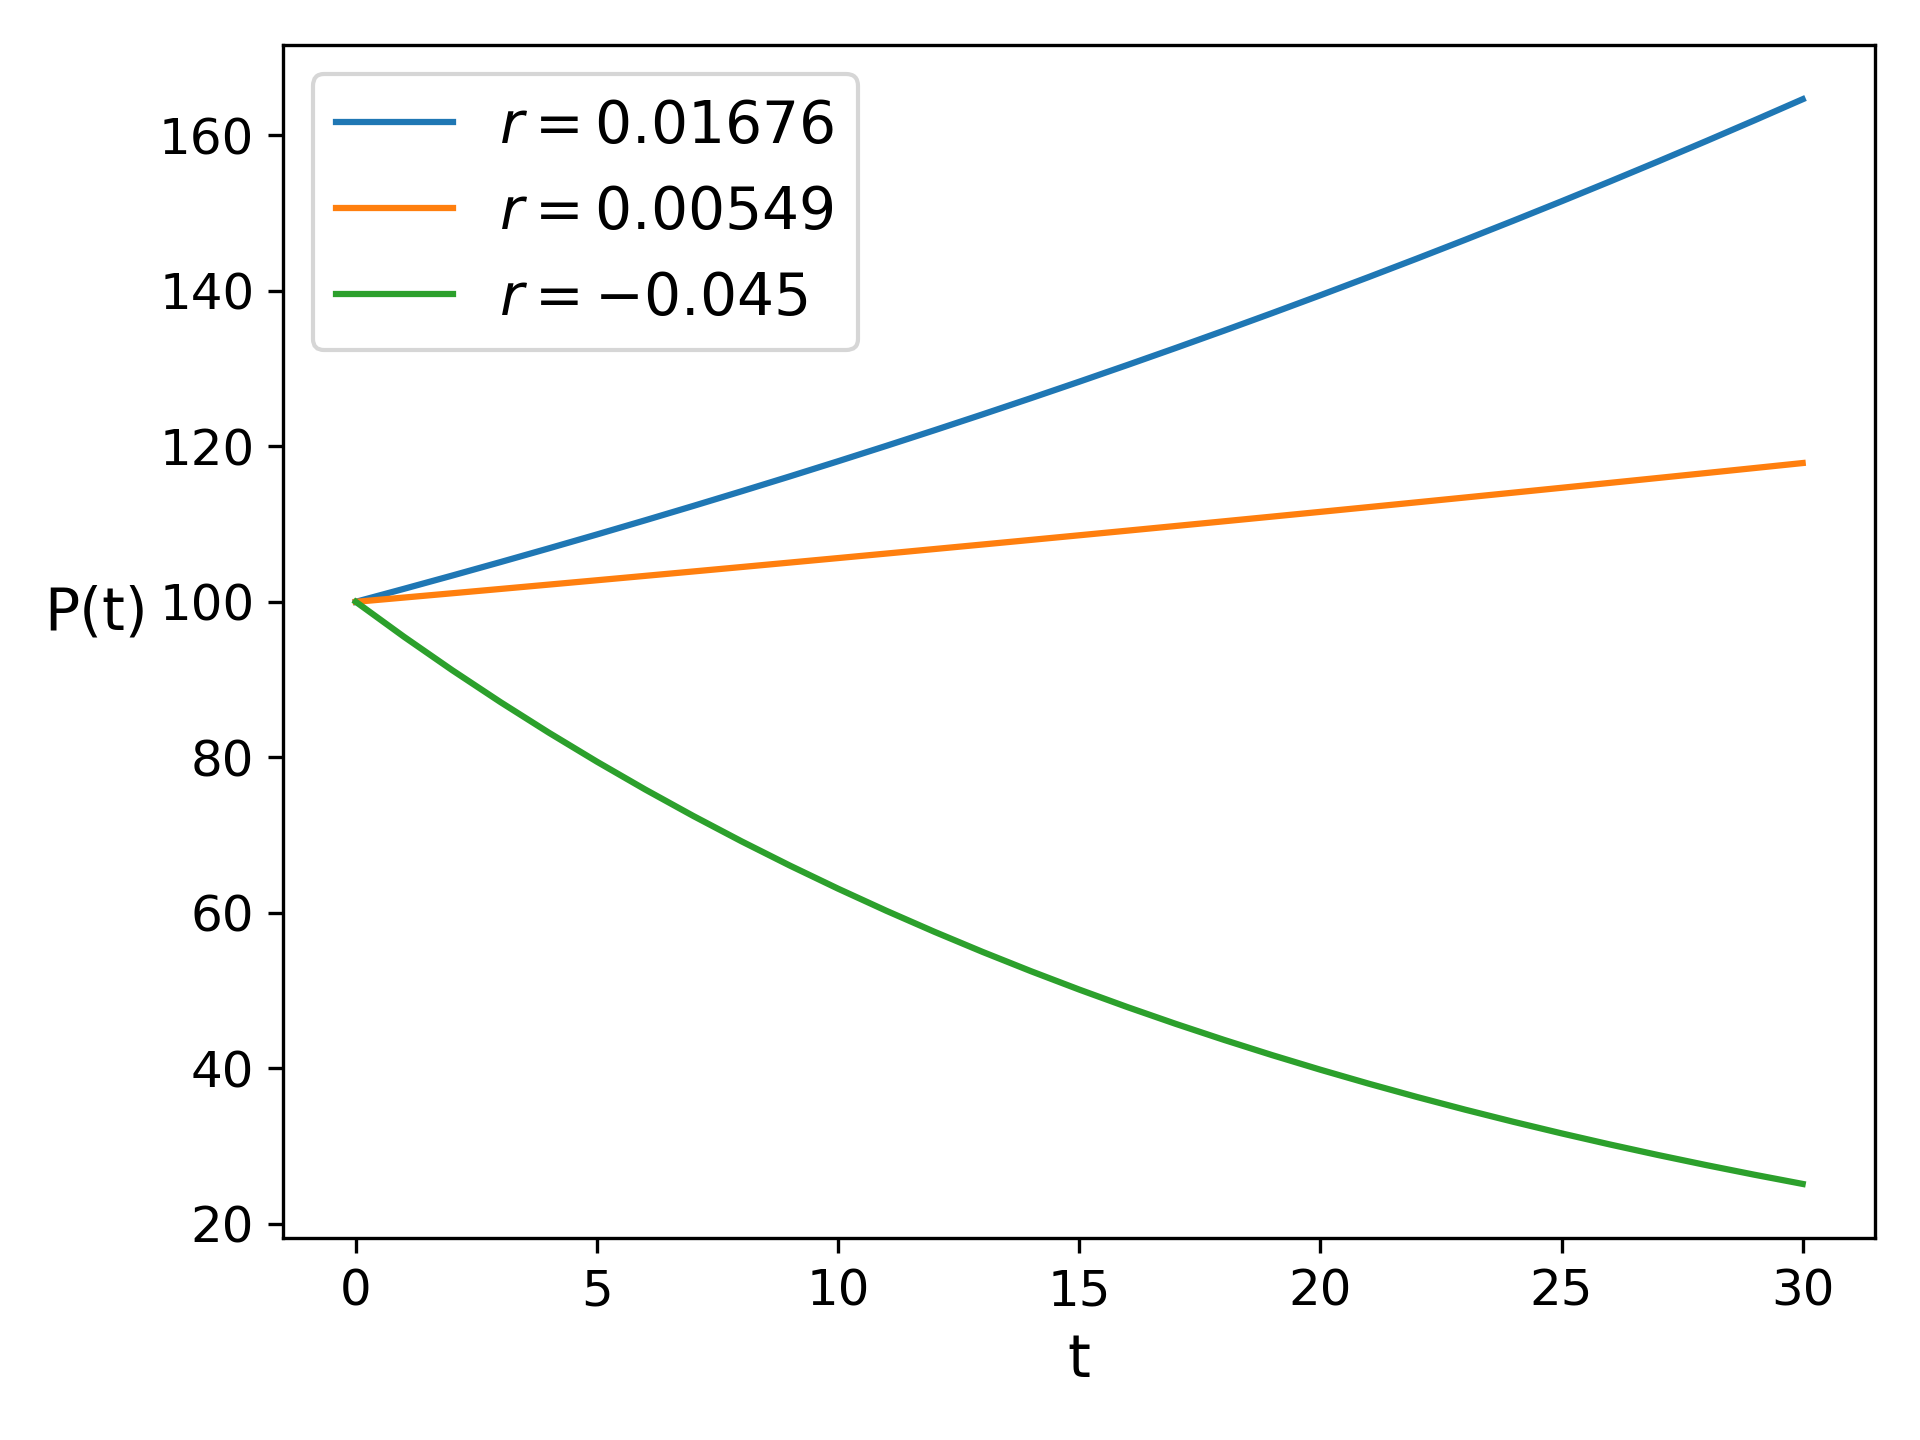
\includegraphics[width=.95\linewidth]{./basic/short_term.png}
        \caption{Bobcat Population over 30 Years}
        \label{fig:basic-short-term}
    \end{subfigure}%
    \begin{subfigure}{.5\textwidth}
        \centering
        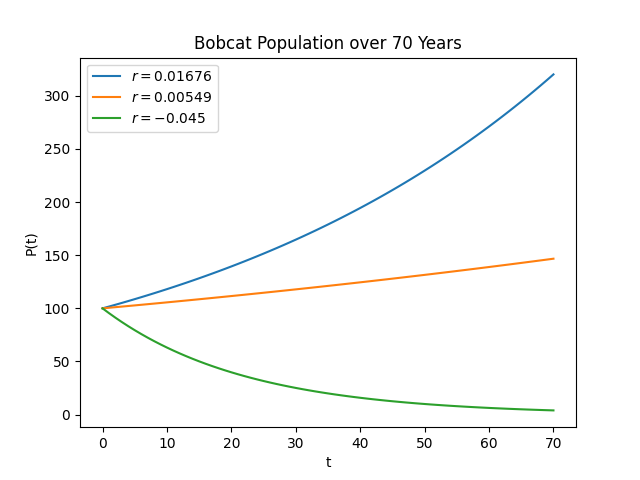
\includegraphics[width=.95\linewidth]{./basic/long_term.png}
        \caption{Bobcat Population over 70 Years}
        \label{fig:basic-long-term}
    \end{subfigure}
    \caption{Bobcat populations in the short (30 year) and long (70 year) term. Using \cref{eq:basic-recursive-exponential} with $P(0) = 100$, and three different growth rates, $r$, being $1.676\%$, $0.549\%$, and $-4.5\%$.}
    \label{fig:1}
\end{figure}

Looking at \cref{fig:1} we can see our exponential behavior. While we're correct in determining how the sign of $r$ effects whether we see growth or decay, we can also see that $r$ is proportional to how fast we grow/ decay, which is inline with our recursive function.

One of the main differences between \cref{fig:basic-short-term} and \cref{fig:basic-long-term} is seeing the speeding up and slowing down of specific lines. In \cref{fig:basic-short-term} it is difficult to tell that the orange and blue lines are growing exponential, while it is immediately obvious that the green line is decaying exponentially. We see a stark change in \cref{fig:basic-long-term}, where it becomes obvious that the orange and blue lines begin to accelerate growth, while the green line slows decay.

This can be mathematically explained. If we recall \cref{eq:basic-closed}, we see that as $t$ increases the number of manipulations by $r + 1$ do as well. If we think of $(r+1)^t$ as the effective growth rate for a specific year applied to the initial population, then we know if $r + 1 > 1$, our effective growth rate will be getting larger. While if $r + 1 < 1$ our effective growth rate will be getting smaller. Thus, a larger effective growth rate will show an acceleration of change, while a smaller effective growth rate will show a slowing of change. This lines up perfectly to the observations we can make about \cref{fig:1}.

This model appears to only have one fixed-point, when $P(t) = 0$, and we only approach this point with negative $r$ values. To confirm this, we can find the derivative of our function at this fixed-point.
\begin{align*}
    P(t) &= (r+1)P(t-1) \\
    P(t) &= f(P(t-1)) \\
    f(x) &= (r+1)x \\
    f'(x) &= r+1
\end{align*}
So referencing \cref{sect:fixed-points}, we know $|f'(x)| < 1$ for a stable fixed-point, and $r+1$ is only less than 1 when $r < 0$. Thus, confirming our claim that $P(t) = 0$ is a stable fixed-point, but only when $r$ is negative. This also means that if $r > 0$, $P(t) = 0$ will be an unstable fixed-point.

With a deep understanding of our incredibly simplistic model we can begin to build on it to add depth and realism.

\section{Hunting}
We now begin to modify our model, assuming we are in best of times, $r = 0.01676$, we will allow hunting. We will introduce two hunting types. First, fixed percentage hunting, i.e. a percentage value $h \ge 0$ is given, as we will hunt that percentage of the population each year. Second, fixed amount hunting, i.e. a specific amount of bobcats $f \ge 0$ is given, and we hunt that amount each year. Finally, we will use the knowledge from these two models to attempt to build a model which allows for a stable population.

\subsection{Percentage Model}
The percentage model is by far the most simple modification to \cref{eq:basic-recursive-exponential}. Given an $h \ge 0$ we get, $P(n) = (1 + r)P(n-1) - hP(n-1)$ simplifying and substituting in $r=0.01676$ to get \cref{eq:hunting-percentage}.
\begin{equation}\label{eq:hunting-percentage}
    P(n) = (r+1-h)P(n-1)
\end{equation}
One may notice, that since $h$ is known beforehand $(r+1-h)$ is simply a constant, just like $(n+1)$ was in \cref{eq:basic-recursive-exponential}. We can solve the recurrence in the same manner as for the basic model, giving us the closed form \cref{eq:hunting-percentage-closed}.
\begin{equation}\label{eq:hunting-percentage-closed}
    P(n) = (r+1-h)^tP(0)
\end{equation}
Since, at this state, this model and the basic model is nearly identical, we can perform the same analysis. If $r < h$, we should expect exponential decay. If $r > h$, we should expect exponential growth. In this case it is possible for $h = r$, this will leave us with a fixed-point at $P(0)$. And from the two previous statements we know this fixed-point must be unstable, as if $r < h$ or $r > h$ we will trend away from it. We also can inherit the fixed point $P(t)=0$, as it will be stable when $r < h$ and unstable when $r > h$.

We will now plot a variety of $h$ values, and see if our analysis lines up to the data. Again we use $P(0)=100$, and as specified above $r = 0.01676$.

\begin{figure}[h]
    \centering
    \begin{subfigure}{.5\textwidth}
        \centering
        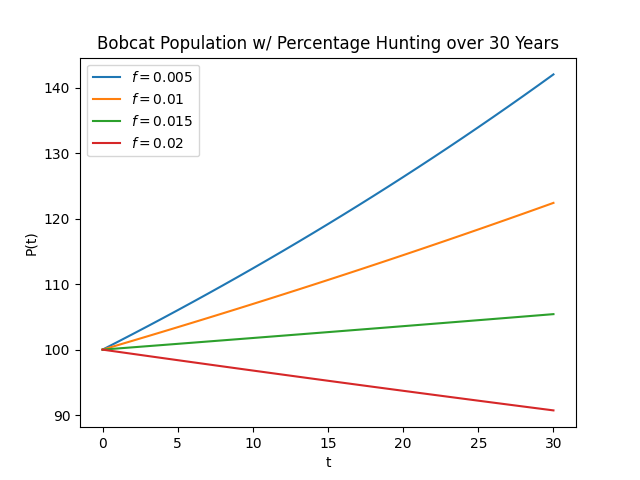
\includegraphics[width=.95\linewidth]{./hunting/percentage_short_term.png}
        \caption{Bobcat Population over 30 Years}
        \label{fig:hunting-percentage-short-term}
    \end{subfigure}%
    \begin{subfigure}{.5\textwidth}
        \centering
        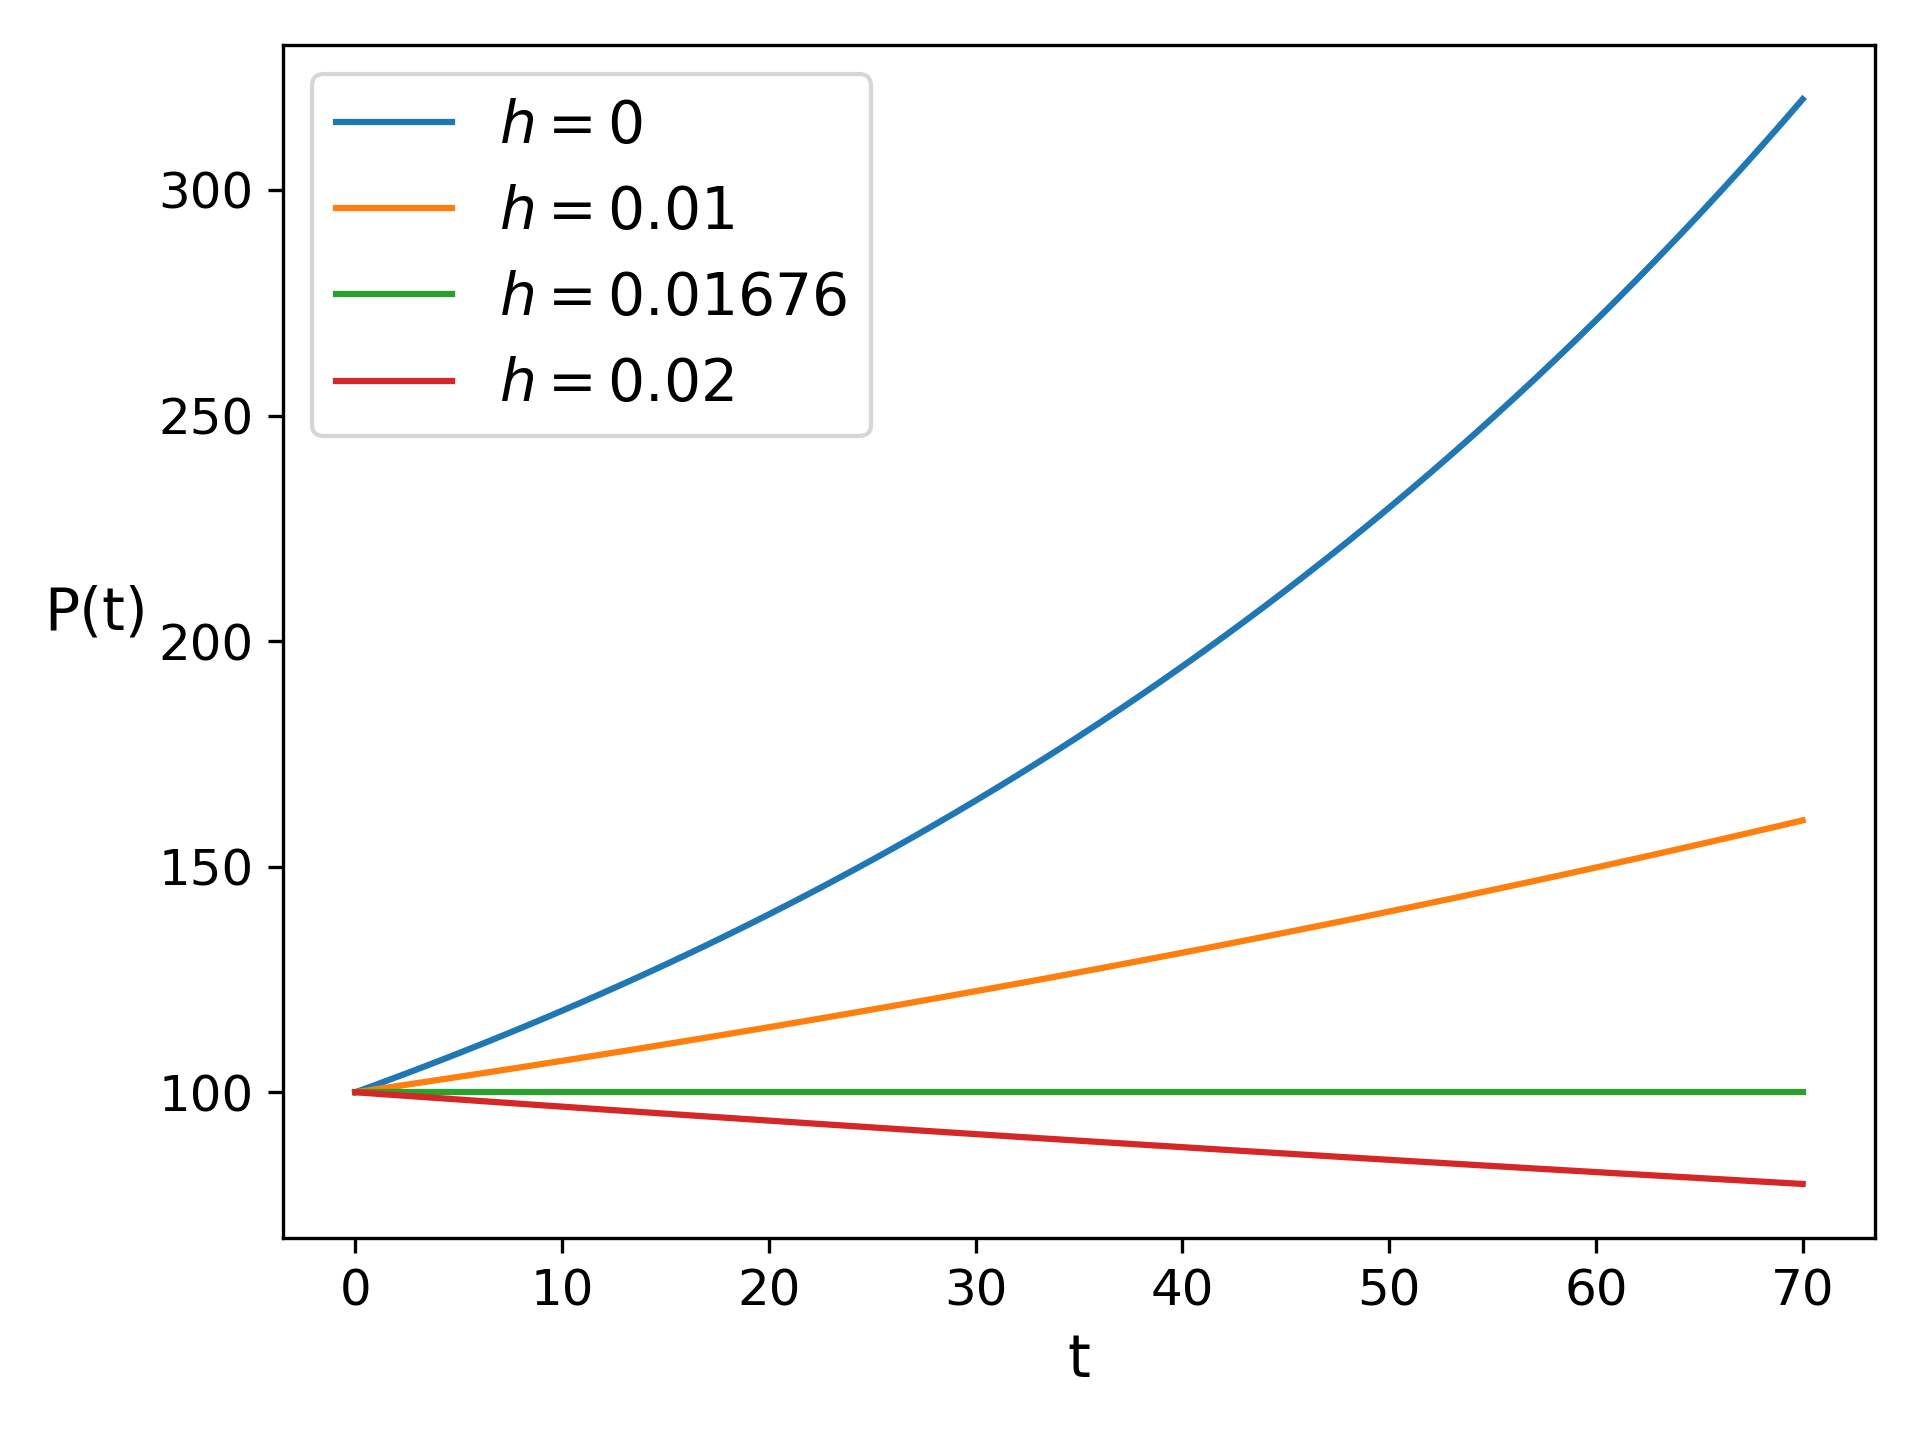
\includegraphics[width=.95\linewidth]{./hunting/percentage_long_term.png}
        \caption{Bobcat Population over 70 Years}
        \label{fig:hunting-percentage-long-term}
    \end{subfigure}
    \caption{Bobcat populations using \cref{eq:hunting-percentage} with $P(0) = 100$, $r = 0.01676$, and four different hunting rates, $h$, being $0\%$, $1.0\%$, $1.676\%$ i.e. $r$, and $2.0\%$.}
    \label{fig:2}
\end{figure}

With a quick glance at \cref{fig:2} we notice it is very similar to \cref{fig:1}. The blue line ($h=0$) is the same on \cref{fig:1} for when $r=0.01676$, as when $h=0$ no hunting is happening. We see that every line where $h > 0$ is below this one, which makes sense. We also see that our predictions held, for the blue and orange lines $h < r$, and we find that these show exponential growth. As expected, we find that when $h=r$ (the green line), we have no change in population and stay at our fixed point. Finally, when $h > r$ (red line) we see exponential decay.

The rest of the analysis on this figure is essentially the same as what we did for the basic model.

\subsection{Amount Model}
The amount model makes some more drastic changes to \cref{eq:basic-recursive-exponential}. We will have some $f \ge 0$ being the amount hunted each year, this forms the recurrence in \cref{eq:hunting-amount}.
\begin{equation}\label{eq:hunting-amount}
    P(n) = (r+1)P(n-1) - f
\end{equation}
While \cref{eq:hunting-amount} looks similar to \cref{eq:hunting-percentage} just with our new variable outside the parenthesis, this vastly changes our closed-form.

\begin{align*}
    P(t) &= (r+1)P(t-1) - f & P(t-1) = (r+1)P(t-2) - f \\
    P(t) &= (r+1)((r+1)P(t-2) - f) - f & P(t-2) = (r+1)P(t-3) - f \\
    P(t) &= (r+1)((r+1)((r+1)P(t-3) - f) - f) - f & P(t-3) = (r+1)P(t-4) - f \\
    &\phantom{x}\vdots \\
    P(t) &= (r+1)^tP(0) - \sum_{k=0}^{t-1}(r+1)^kf
\end{align*}
With the last term, the summation, we can apply the geometric series formula(\cref{eq:geometric-series}).
\begin{equation*}
    \sum_{k=0}^{t-1}(r+1)^kf = f\frac{(r+1)^t-1}{r+1-1}
\end{equation*}
Which we can then substitute this in, to get the full closed-form.
\begin{equation}\label{eq:hunting-amount-closed}
     P(t) = (r+1)^tP(0)-f\frac{(r+1)^t-1}{r}
\end{equation}

\Cref{eq:hunting-amount-closed}, however different from previous equations, is still an exponential function. Meaning we can continue to use the same analysis tools. First we can attempt to find the points at which we change from exponential growth to decay. To do so let's solve for the change from the one year to the next.
\begin{align*}
    P(1) &= (r + 1)P(0)-f \\
    P'(1) &= (r + 1)P(0) - f - P(0) \\
    P'(1) &= rP(0)+P(0)-f-P(0) \\
    P'(1) &= rP(0) - f
\end{align*}

While this looks similar to when we have calculated this for the previous models, there is one major change. We can no longer ignore $P(0)$ when determining the sign. In fact, we must use the entire expression to determine sign. So $\sgn(P'(1)) = \sgn(rP(0)-f)$. For \cref{eq:basic-recursive-exponential} we knew our sign only relied on $r$, for \cref{eq:hunting-percentage} we knew our sign relied on $r$ and $h$. In this case we rely on three things, the initial population, the growth rate, and the hunting amount. For the previous equations our analysis could hold, no matter the initial population, now we must be very careful to take the initial population into account.

In this scenario we can start by keeping this generic, then we can introduce our known values for $r$ and $P(0)$ to calculate the actual points where behavior will change. We expect to see exponential growth when $rP(0)>f$, we should see decay when $rP(0)<f$, and should see no growth or decay when $rP(0)=f$.

Previously we have two fixed-points, one at the initial population, and one at zero. While, the initial population fixed-point still makes sense, the zero fixed-point no longer does. If we take \cref{eq:hunting-amount-closed} at $P(0)=0$, we will get $P(t) = -f\frac{(r+1)^t}{r}$, and we assume $r > 0$, we will get a negative exponential. And since we are already at 0, this function will not be asymptotic, but instead see negative exponential growth, which is something we have not seen. This means instead of having a standard exponential decay, where our function slows as it approaches 0, we will actually see the function speed up past zero.

Now, let's analyze our inflection points with the known variables $P(0) = 100$ and $r = 0.01676$. We can then use our inequalities from earlier. If $1.676<f$ we should see, not exponential decay, but negative exponential growth. If $1.676>f$ then we will see exponential growth. In the case of $f=1.676$ we would see our stable fixed-point at $P(t)=100$, but this is one of the cases where asking people to hunt a decimal of a bobcat is unrealistic.

\begin{figure}[h]
    \centering
    \begin{subfigure}{.5\textwidth}
        \centering
        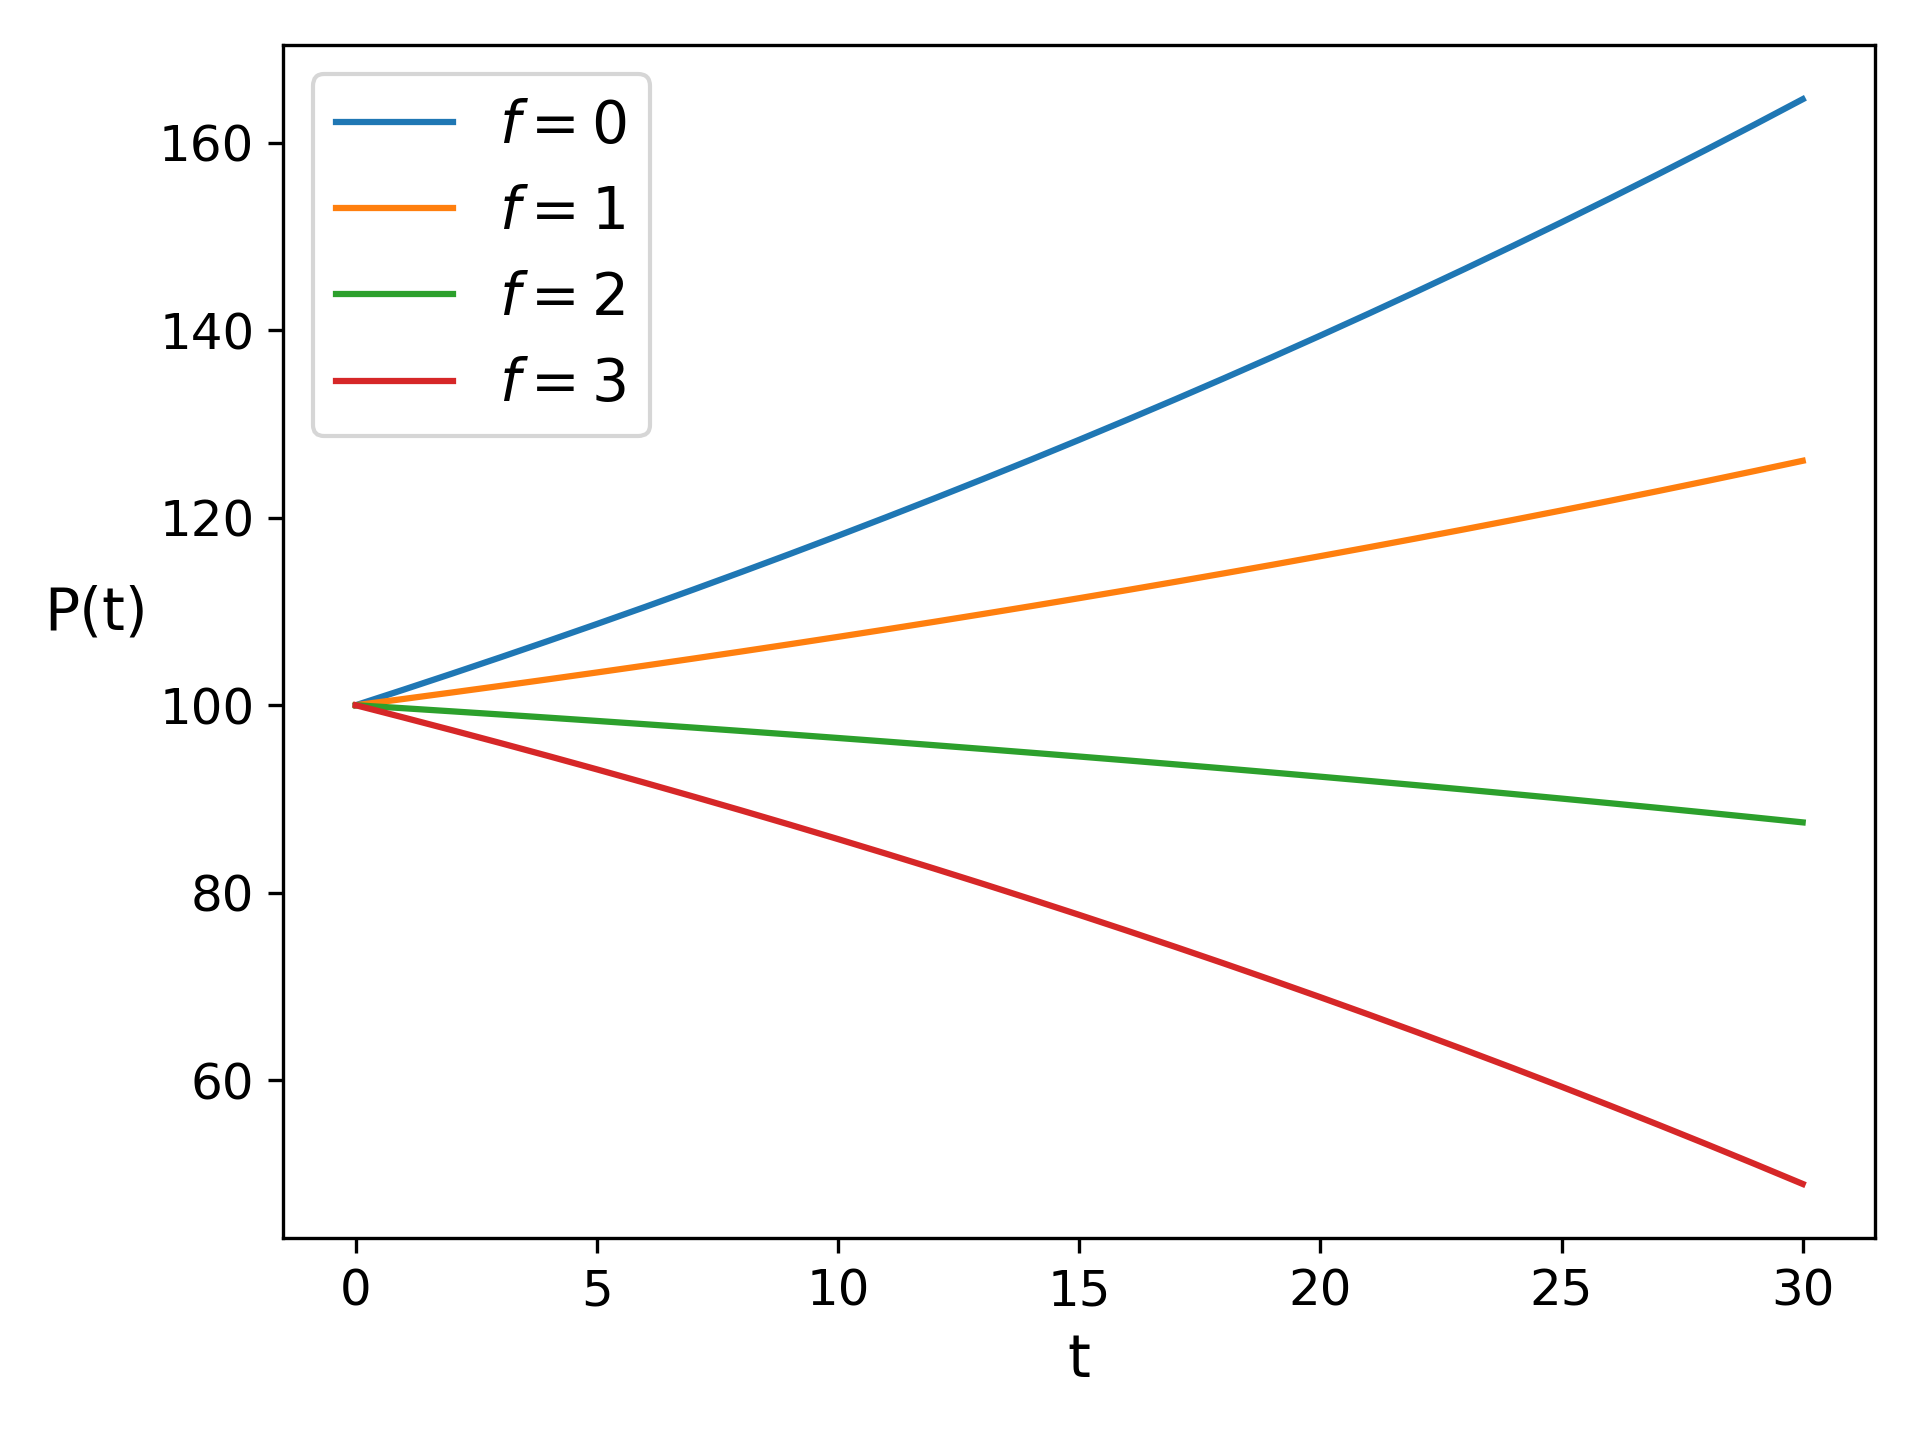
\includegraphics[width=.95\linewidth]{./hunting/amount_short_term.png}
        \caption{Bobcat Population over 30 Years}
        \label{fig:hunting-amount-short-term}
    \end{subfigure}%
    \begin{subfigure}{.5\textwidth}
        \centering
        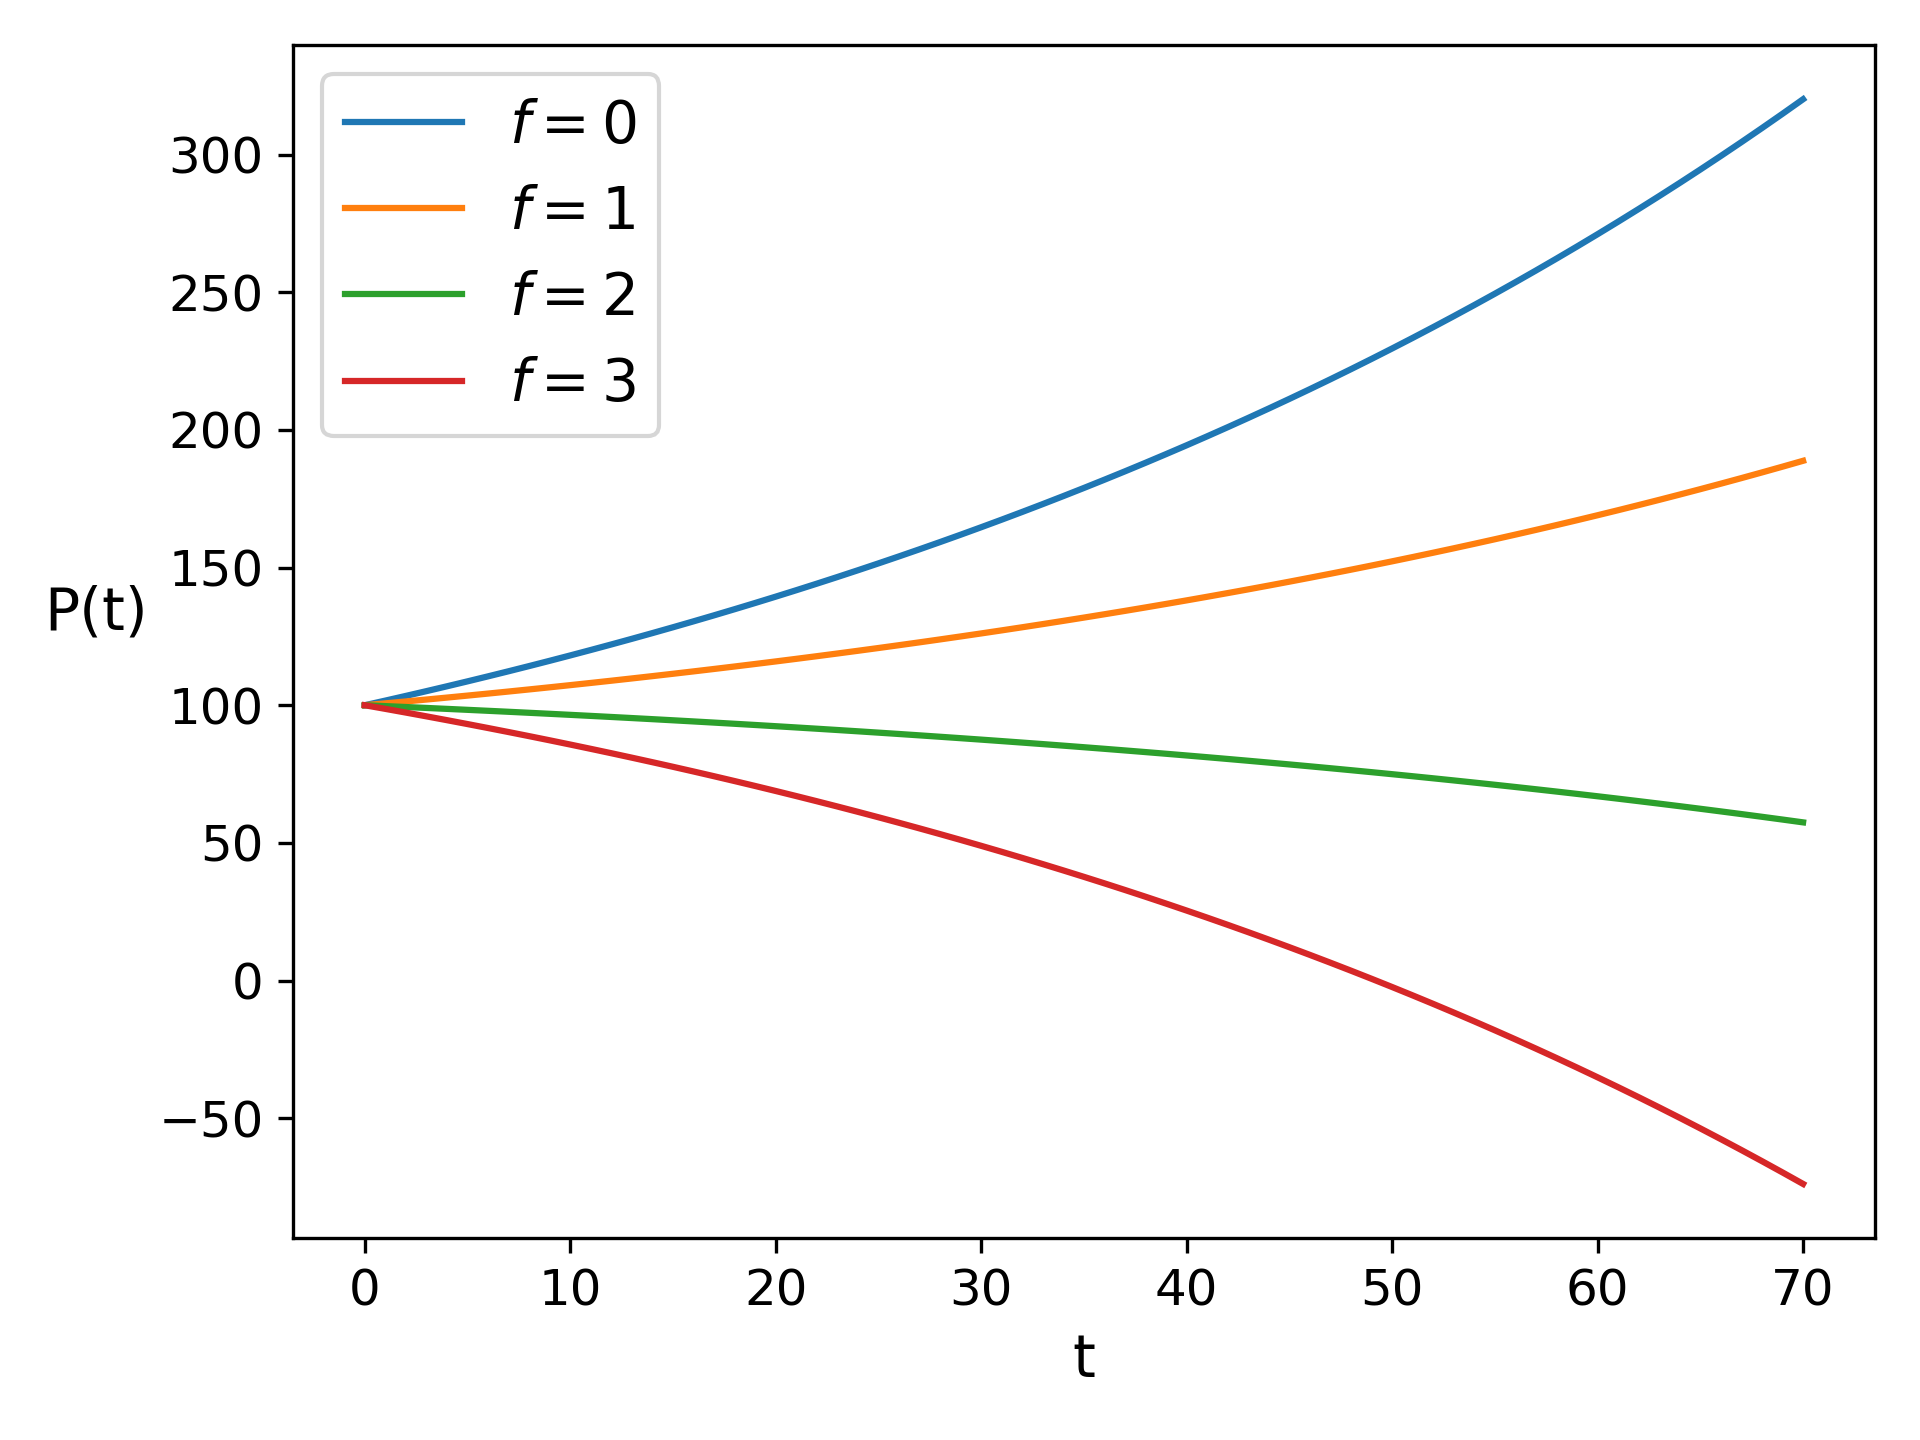
\includegraphics[width=.95\linewidth]{./hunting/amount_long_term.png}
        \caption{Bobcat Population over 70 Years}
        \label{fig:hunting-amount-long-term}
    \end{subfigure}
    \caption{Bobcat populations using \cref{eq:hunting-amount} with $P(0) = 100$, $r = 0.01676$, and four different fixed hunting amounts, $f$, being 0, 1, 2, and 3.}
    \label{fig:3}
\end{figure}

Looking at \cref{fig:3}, it does not look similar to \cref{fig:1,fig:2}. Similar to those we can see how in \cref{fig:hunting-amount-short-term} it is difficult to see the exponential growth or decay, but then looking at \cref{fig:hunting-amount-long-term} we can see the functions speed up. The main difference, as talked about previously, there is no exponential decay, instead we see both positive and negative exponential growth.

Our expectations were met, as when $f=0,1$, i.e. $f < 1.676$, we saw a positive rate of change, and when $f=2,3$, i.e. $f > 1.676$, we saw a negative rate of change. This model is also the first model to introduce negative populations, which doesn't make much sense realistically. While this model introduced complexity, and new behaviors (negative exponential growth), we were able to apply the same techniques as we have on the previous models, and get accurate results.

\subsection{Stable Model}
For this section we have the goal of devising a strategy to have the population increase to around 200 bobcats, then remain roughly constant over time. We continue to use $P(0)=100$ and $r = 0.01676$. We can devise this strategy with either of our two models, or with both of them.

Neither of our two models have stable fixed points, which means we can't solve for a fixed point at $P(t)=200$ and have our population rise to it. Instead, we can use what we have learned in the analysis of our methods. For our fixed percentage hunting model, \cref{eq:hunting-percentage}, we know that if $r > h$, we can expect exponential growth. We can use this fact to let us grow up to the population we want. Since $r = 0.01676$, any $h$ value less than this will allow for growth at different rates. For our fixed amount hunting model, \cref{eq:hunting-amount}, we know that when $rP(0) > f$ we will see exponential growth.

\begin{figure}[h]
    \centering
    \begin{subfigure}{.5\textwidth}
        \centering
        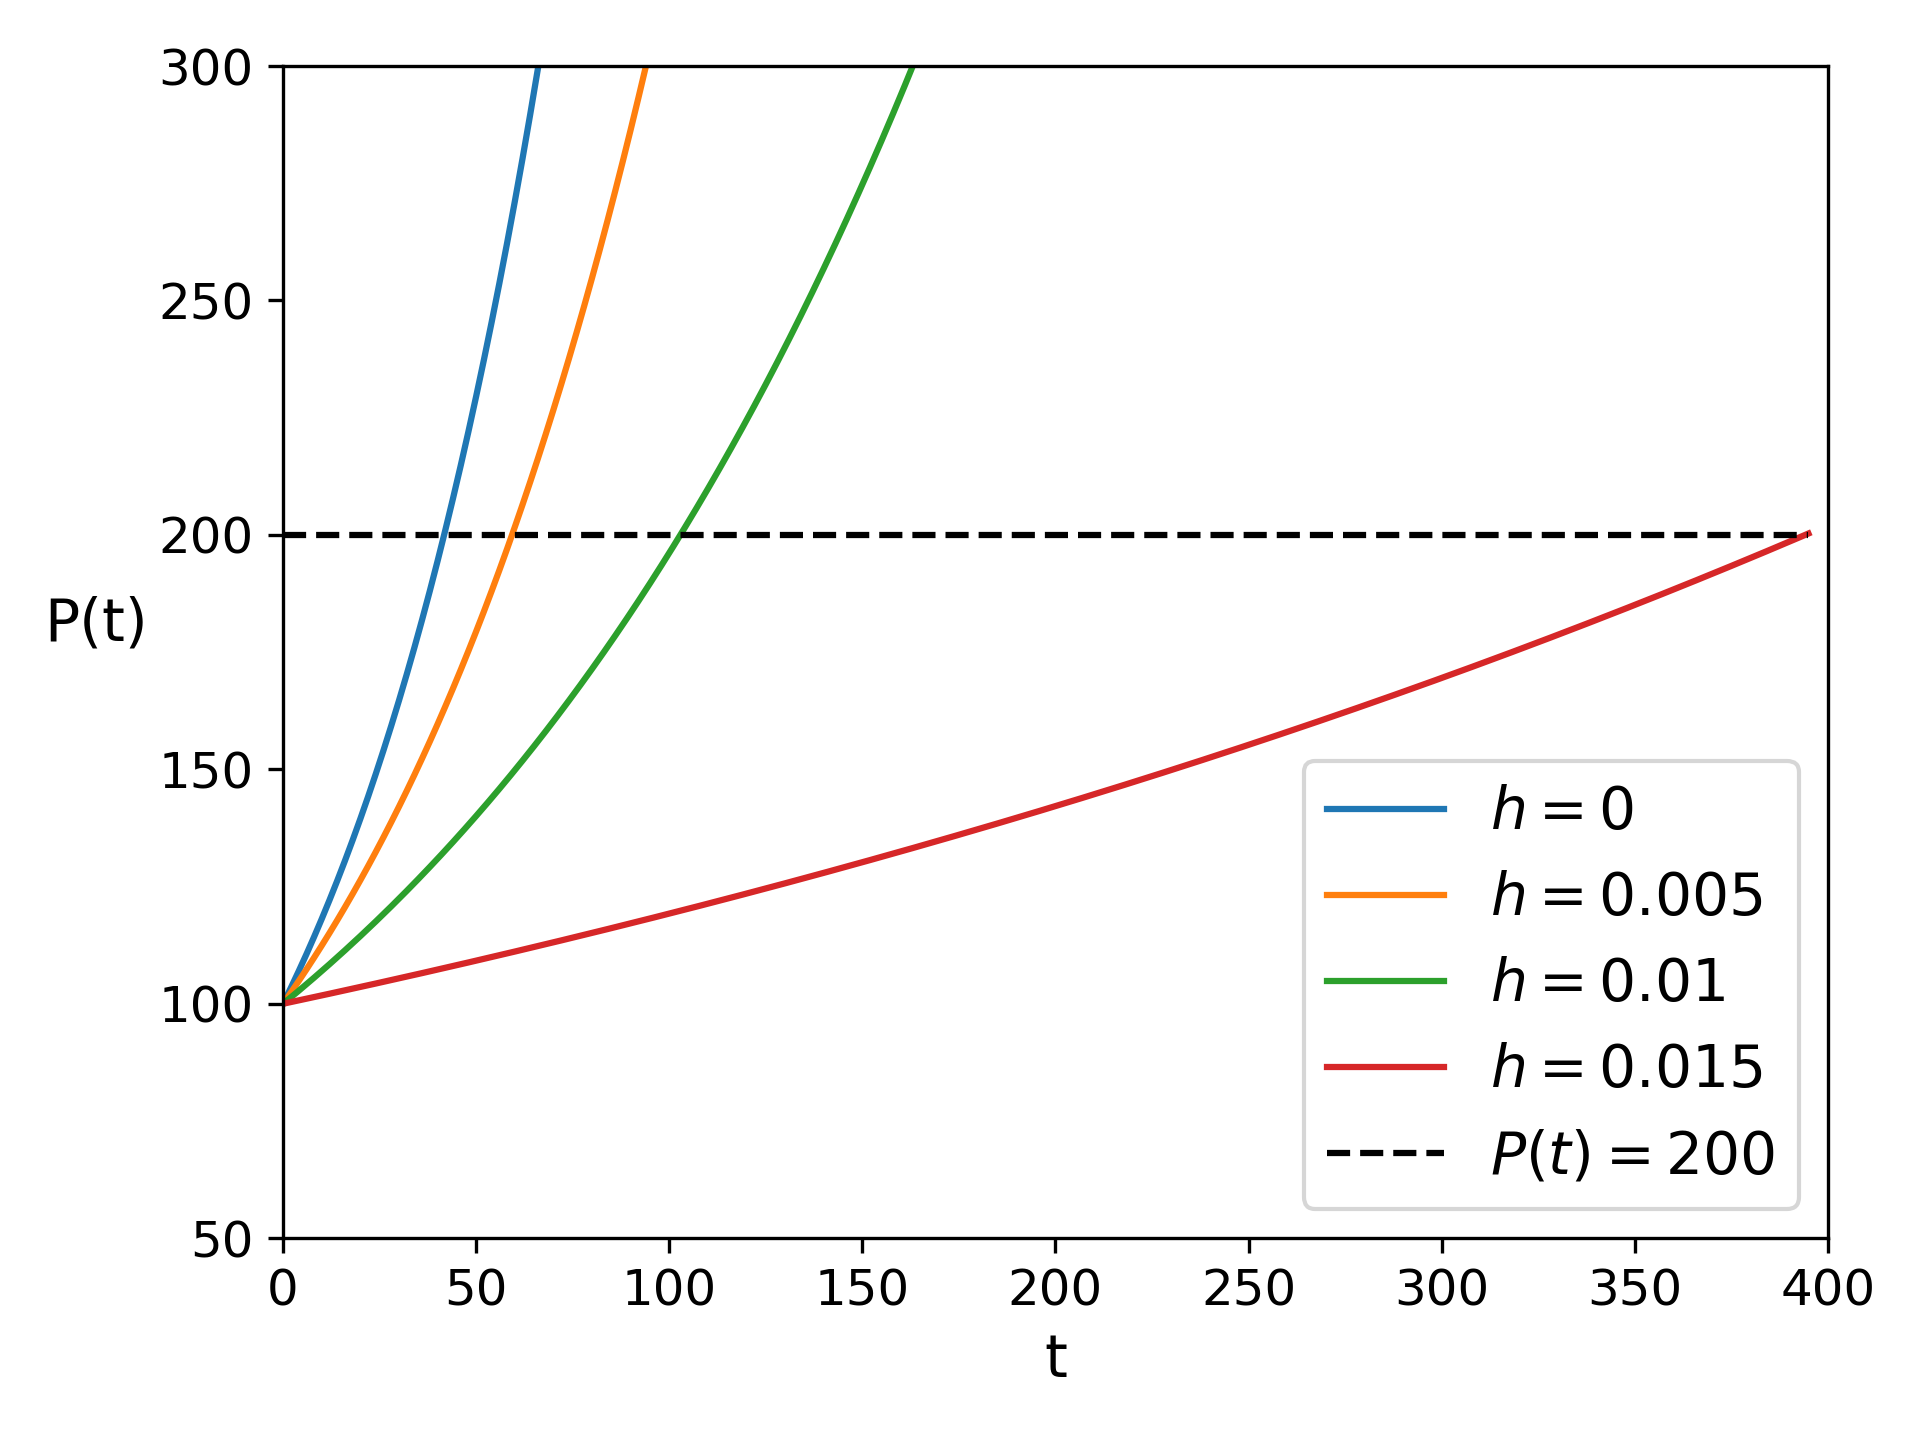
\includegraphics[width=.95\linewidth]{./hunting_strategy/percentage_growth.png}
        \caption{Population using \cref{eq:hunting-percentage}}
        \label{fig:hunting-strategy-percentage-growth}
    \end{subfigure}%
    \begin{subfigure}{.5\textwidth}
        \centering
        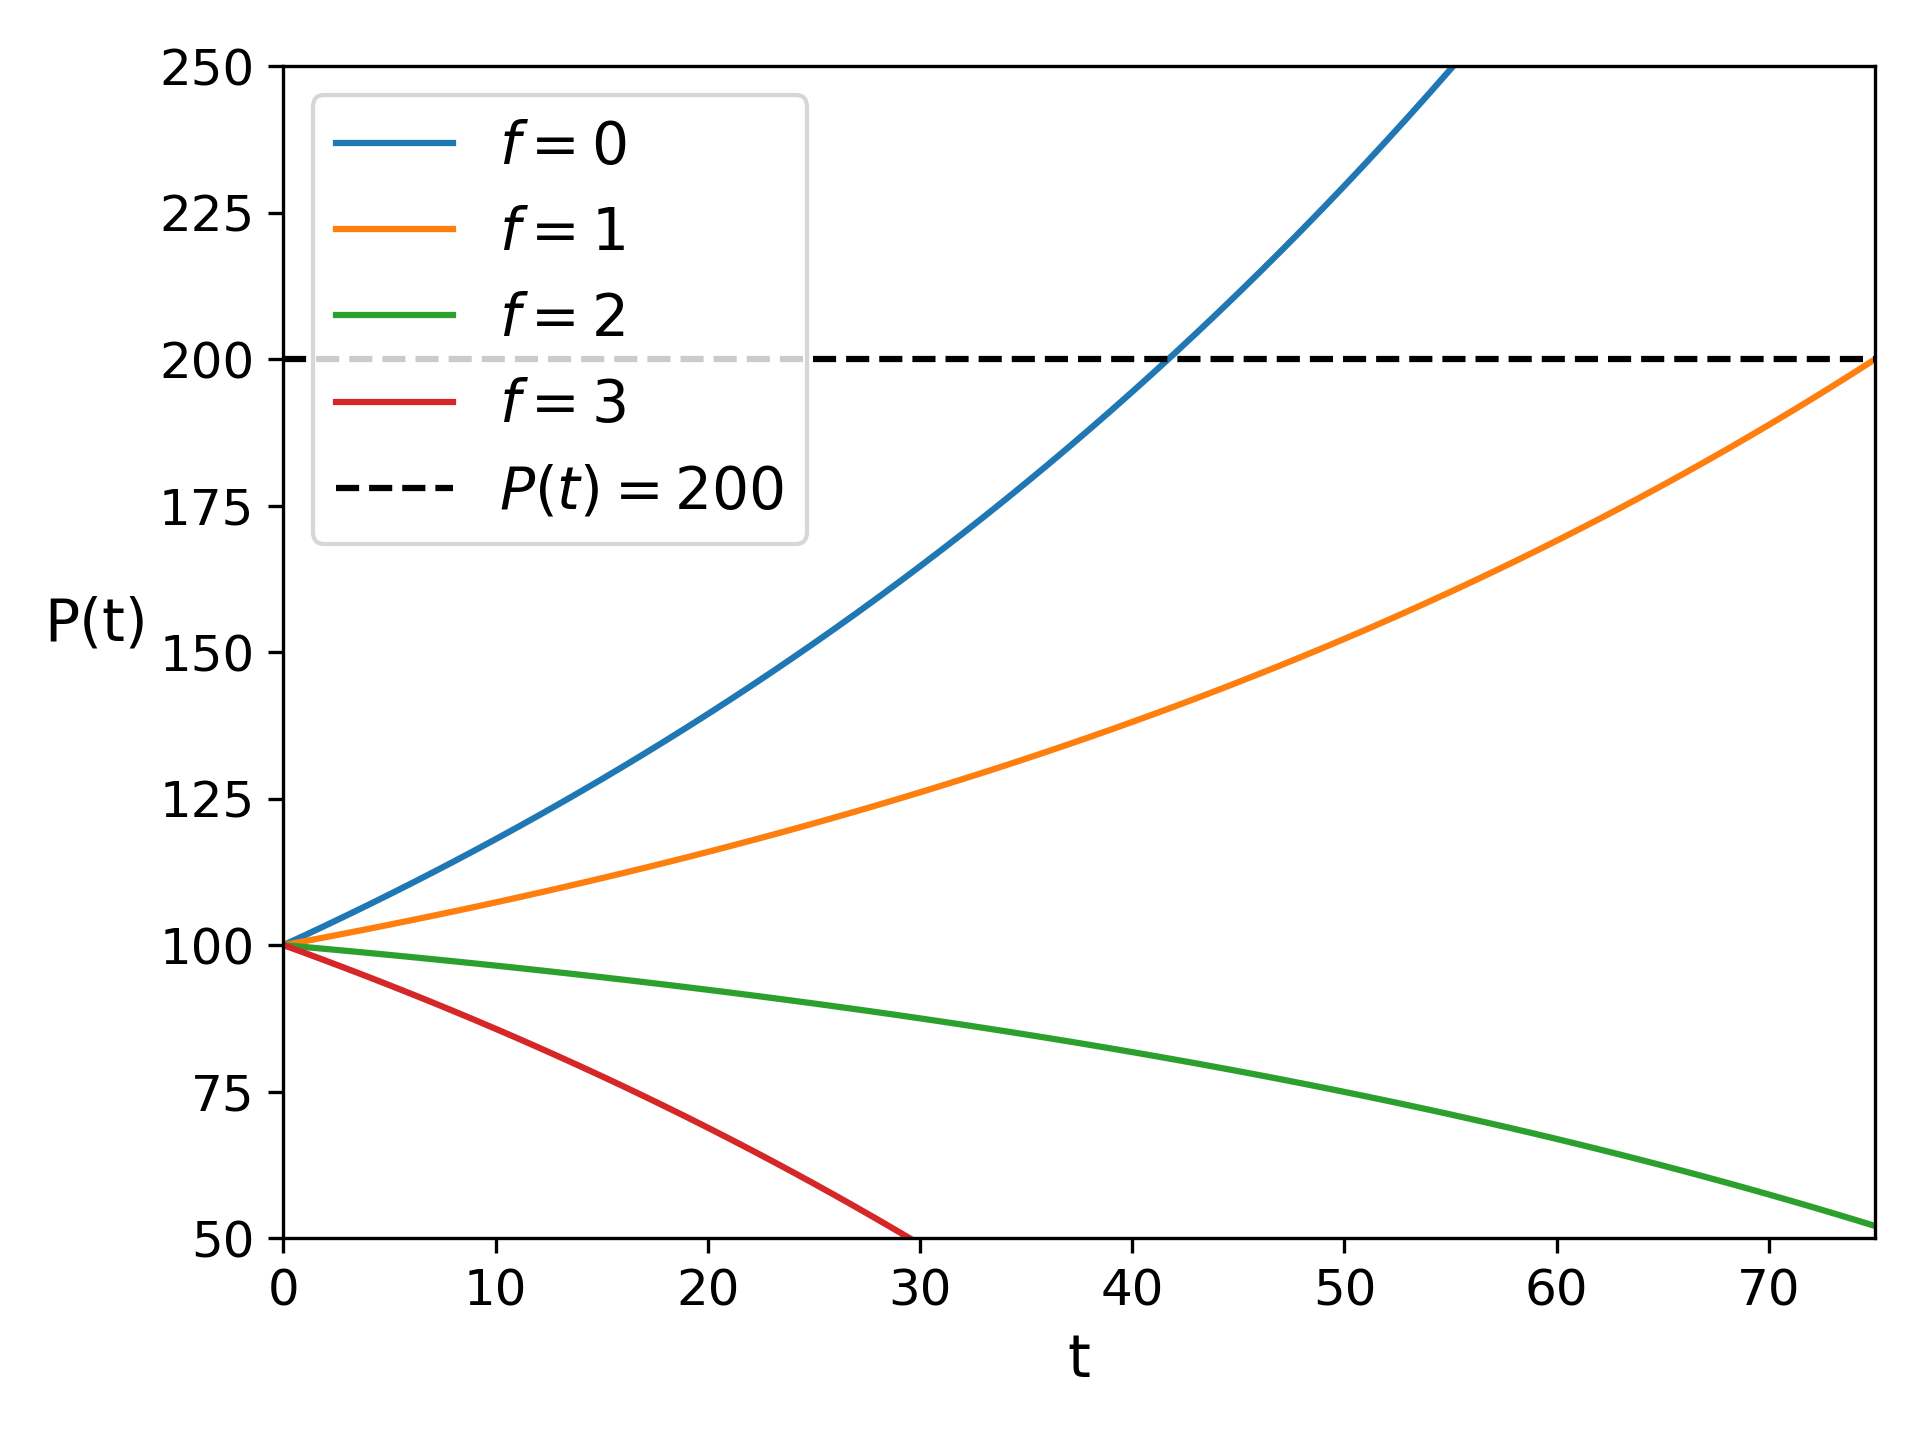
\includegraphics[width=.95\linewidth]{./hunting_strategy/amount_growth.png}
        \caption{Population using \cref{eq:hunting-amount}}
        \label{fig:hunting-strategy-amount-growth}
    \end{subfigure}
    \caption{Bobcat populations using \cref{eq:hunting-percentage} and \cref{eq:hunting-amount} with $P(0) = 100$ and $r = 0.01676$. Highlighting how each grows to $P(t)=200$ given different parameters.}
    \label{fig:4}
\end{figure}

In \cref{fig:4} we can see how each of these models grows to 200. Looking at \cref{fig:hunting-strategy-amount-growth}, we see only two values of $f$ work, as $rP(0) > f$ with our $r$ and $P(0)$ is $1.676 > f$. So only 0 and 1 will work for a real world hunting amount, everything higher will cause the population to decrease. \Cref{fig:hunting-strategy-percentage-growth} shows that there are many more values that work. Since we simply need $h < 0.01676$, any decimal value between $0$ and $0.01676$ works. In both \cref{fig:hunting-strategy-percentage-growth,fig:hunting-strategy-amount-growth} the blue line represents the same function, modeled by our basic model in  \cref{eq:basic-recursive-exponential}, as no hunting is happening. We can see a definite advantage to using \cref{eq:hunting-percentage} initially, as it will give us many more ways to reach $P(t)=200$.

We can find when our population will reach 200 by using the closed-form \cref{eq:hunting-percentage-closed}. Then solving for $t$. For the sake of numerical simplicity, since we know the constants values, we will use them.
\begin{align*}
    200 &= 100(1.01676-h)^t \\
    2 &= (1.01676-h)^t \\
    \log_{1.01676-h}(2) &= t
\end{align*}
The form above will give us a decimal year result, which we know will not work. If we use less than our calculated population won't quite reach 200, so instead we will use the ceiling of this result. \Cref{eq:hunting-strategy-time} gives us the year we will have hit 200 population, when $P(0) = 100$ and $r = 0.01676$, for any $h$. Using this, we can find that if $h=0.01$, for example, $P(t) = 200$ once $t = 103$.

\begin{equation}\label{eq:hunting-strategy-time}
    \tau(h) = \lceil\log_{1.01676-h}(2)\rceil
\end{equation}

Once our population has hit $P(t)=200$, we can adjust our model to allow for population stability. While we could continue to use \cref{eq:hunting-percentage}, its stability happens when $h=r$, i.e. the model becomes our basic model \cref{eq:basic-recursive-exponential}. Instead, we will use our fixed amount model to maintain stability. With our analysis of \cref{eq:hunting-amount} we found that it will be stable when $P(0)r = h$. In this case our model will begin when the population has hit 200, so $200r=h$. And we know that $r = 0.01676$ giving us a stable hunting amount of $3.352$.

The issue is that this hunting amount does not make much sense in the real world, as hunting 0.352 of a bobcat would have to be done. Instead, we can alternate between a hunting amount of $3$ and $4$. We can do this depending on the previous year's population. If $P(t-1) > 200$, we use $4$, which causes a negative growth rate. If $P(t-1) \le 200$, we use $3$, which causes a positive growth rate. This will allow our population to remain close to $200$ once reaching it.

We can create a formal piece-wise function of this model combining \cref{eq:hunting-percentage,eq:hunting-amount,eq:hunting-strategy-time} to get \cref{eq:hunting-strategy-model}.
\begin{equation}\label{eq:hunting-strategy-model}
P(t) =
    \begin{cases}
        (r+1-h)P(t-1)  & \text{if } t \le \tau(h) \\
        (r+1)P(t-1) + 3& \text{if } t > \tau(h) \text{ and } P(t-1) \le 200 \\
        (r+1)P(t-1) + 4& \text{if } t > \tau(h) \text{ and } P(t-1) > 200 \\
    \end{cases}
\end{equation}

\begin{figure}[h]
    \centering
    \begin{subfigure}{.5\textwidth}
        \centering
        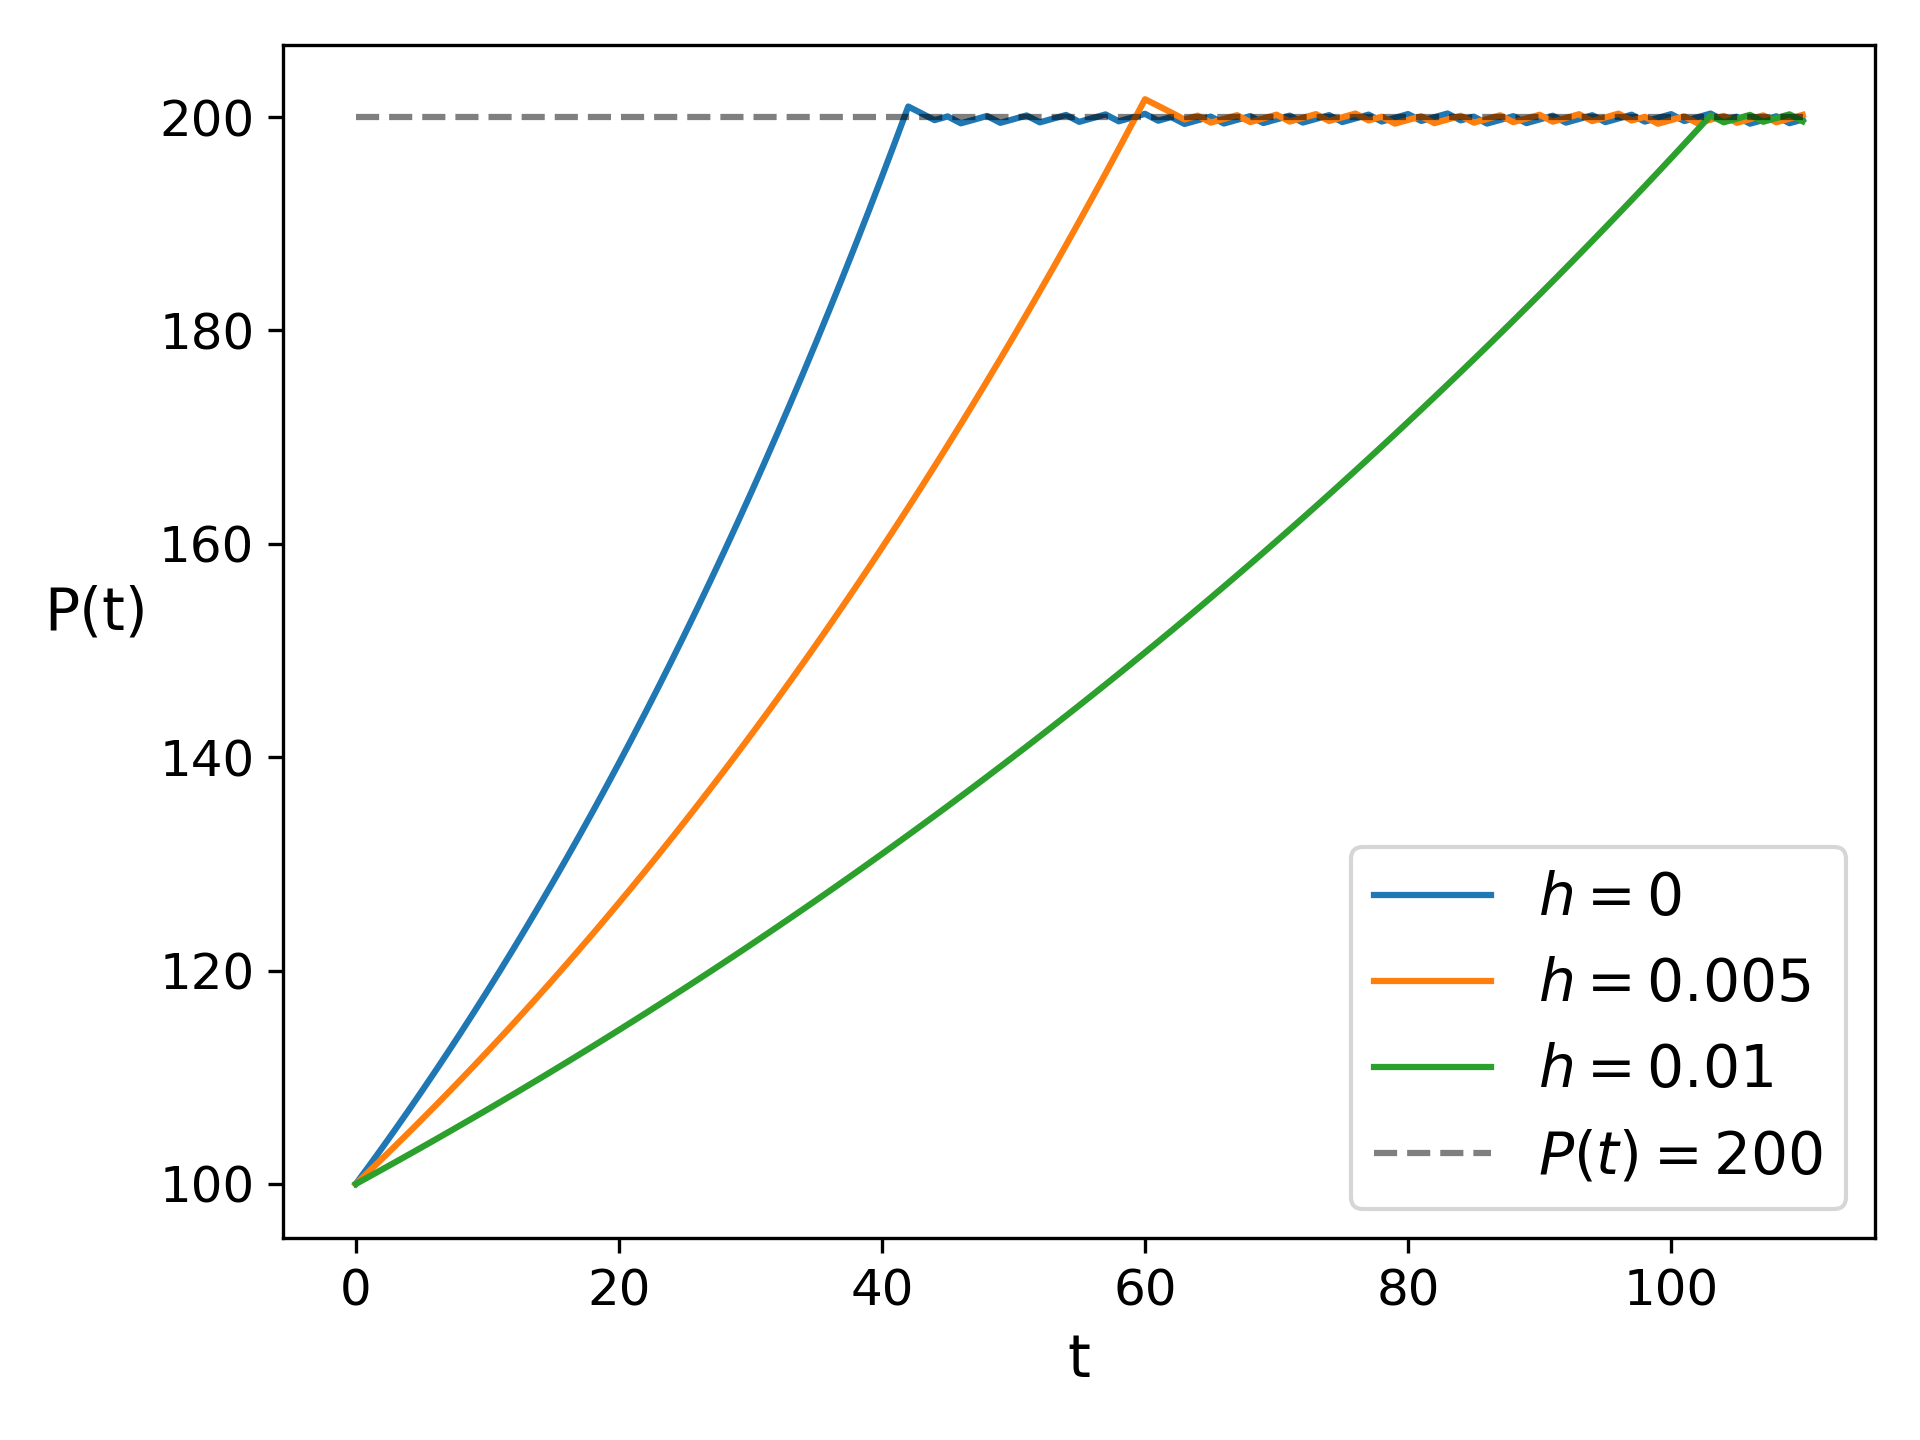
\includegraphics[width=.95\linewidth]{./hunting_strategy/strategic_model_short_term.png}
        \caption{Bobcat Population over 110 Years}
        \label{fig:hunting-strategy-model-short-term}
    \end{subfigure}%
    \begin{subfigure}{.5\textwidth}
        \centering
        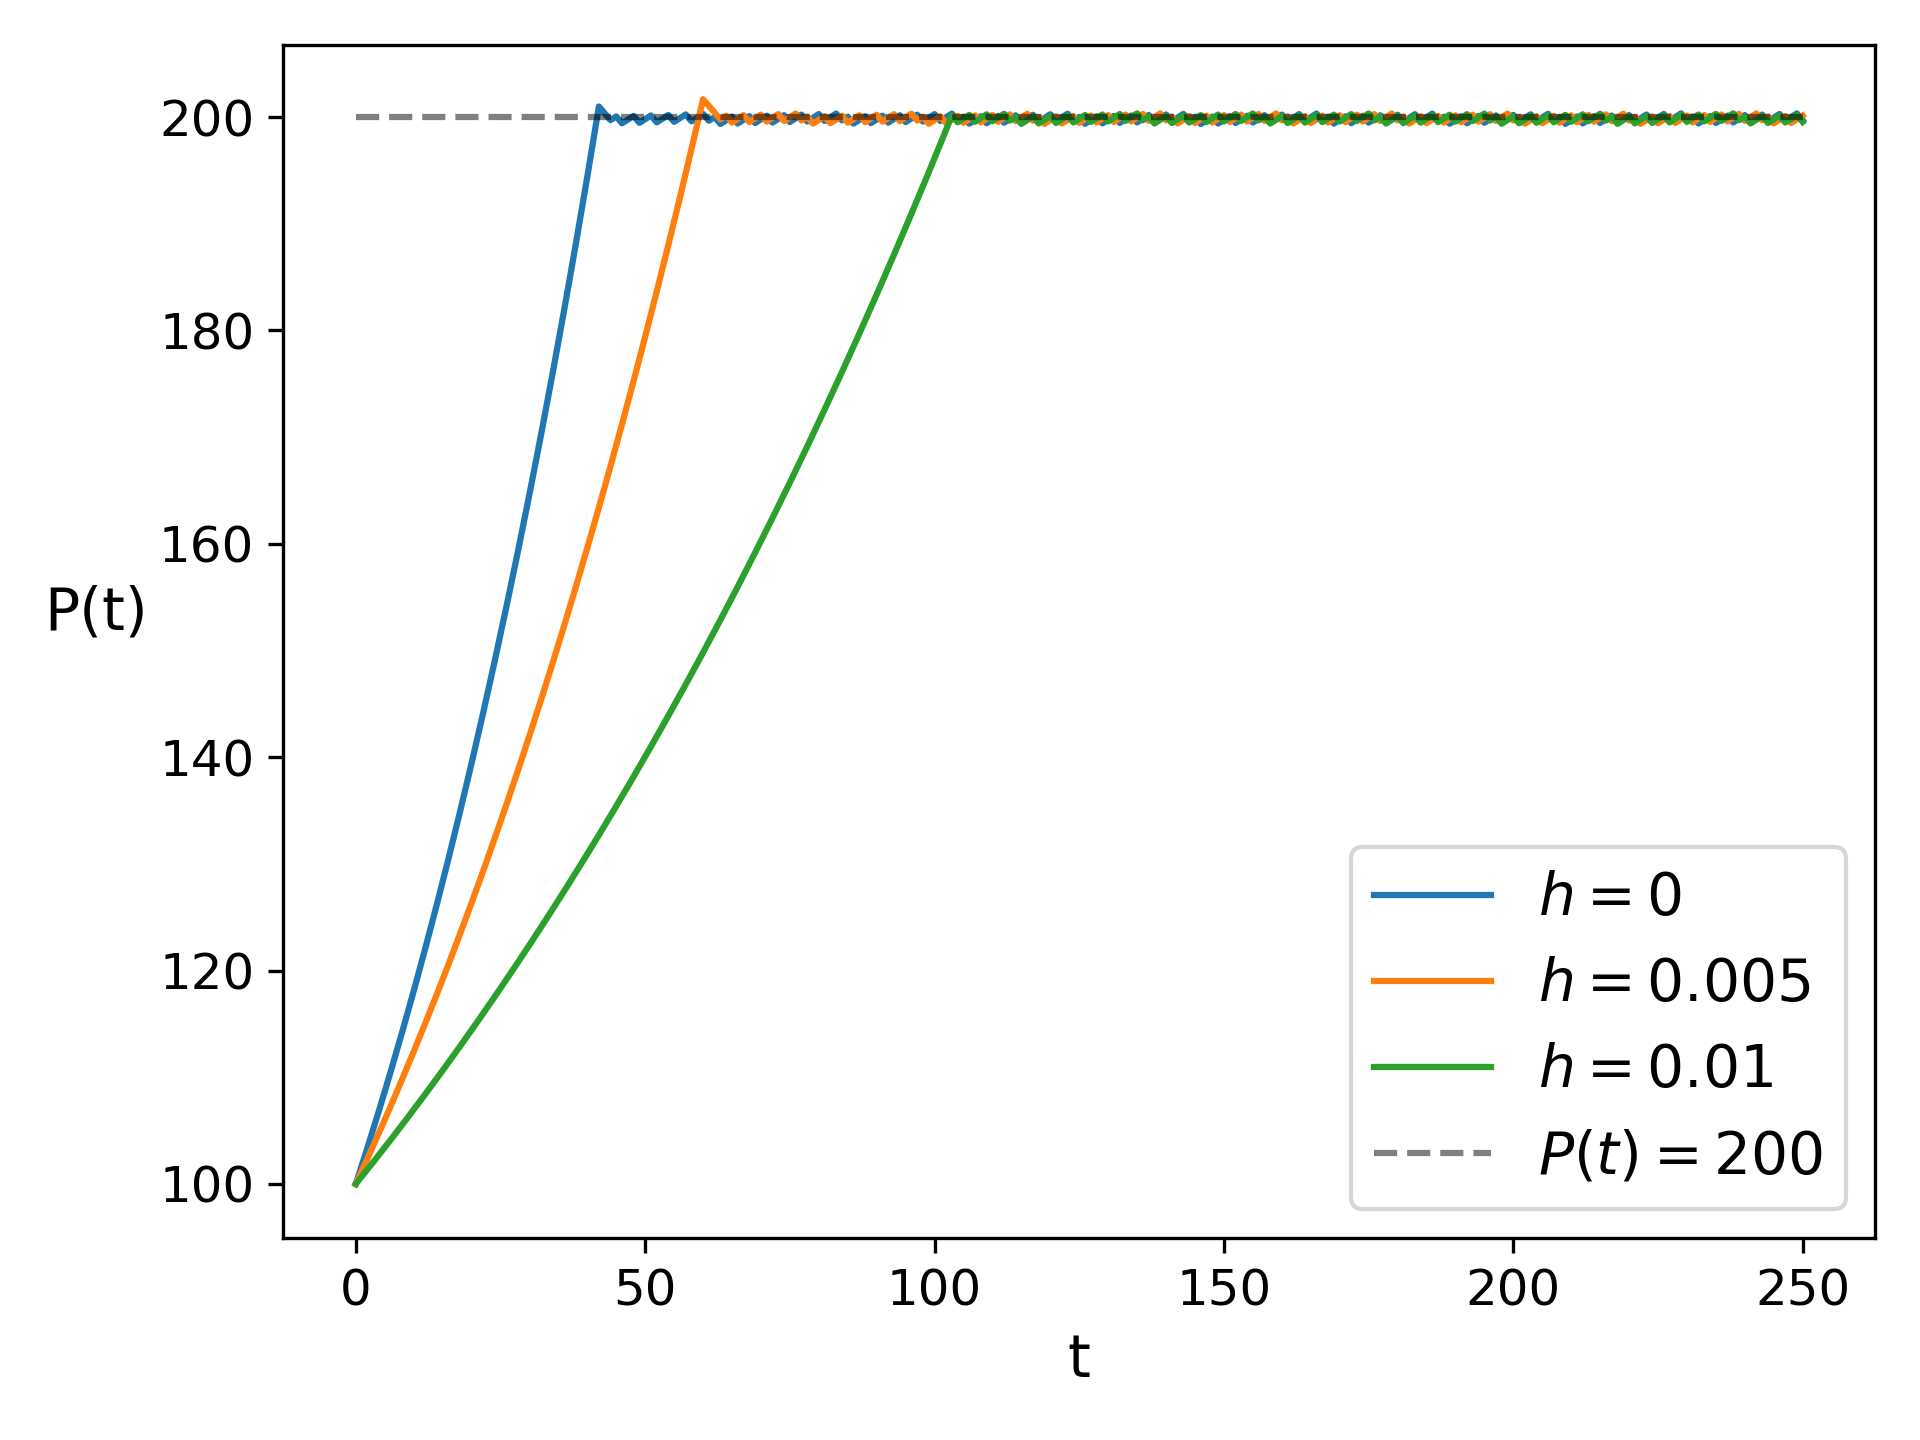
\includegraphics[width=.95\linewidth]{./hunting_strategy/strategic_model_long_term.png}
        \caption{Bobcat Population over 250 Years}
        \label{fig:hunting-strategy-model-long-term}
    \end{subfigure}
    \caption{Bobcat populations using the strategic model \cref{eq:hunting-strategy-model} with $P(0) = 100$ and $r = 0.01676$.}
    \label{fig:5}
\end{figure}

In \cref{fig:5} we can see how our strategic model works in the short and long term. \Cref{fig:hunting-strategy-model-long-term} shows how effective it is, as even after 250 years, no matter what $h$ is used for initial growth, we remain at a population of 200. As expected, the value of $h$ only changes how quickly we reach 200. We can say our model is successful in reaching and maintaining a stable population of 200.

\end{document}